%!TEX program = xelatex
\documentclass{beamer}

\usepackage[english]{babel}

\usepackage{graphicx,hyperref,url, materialbeamer}
\usepackage{braket}
\usepackage{euler}
\usepackage{listings}


\graphicspath{ {./figs/} }
\setbeamercovered{transparent}
\lstdefinestyle{customsql}{
  belowcaptionskip=1\baselineskip,
  breaklines=true,
  xleftmargin=\parindent,
  language=SQL,
  showstringspaces=false,
  basicstyle=\footnotesize\ttfamily,
  keywordstyle=\bfseries\color{green!40!black},
  commentstyle=\itshape\color{purple!40!black},
  identifierstyle=\color{blue},
  stringstyle=\color{orange},
}
\lstset{escapechar=@,style=customsql}



\usefonttheme{professionalfonts} % using non standard fonts for beamer
%\usefonttheme{serif}

% The title of the presentation:
%  - first a short version which is visible at the bottom of each slide;
%  - second the full title shown on the title slide;
\title[Parallel and Continuous Join Processing for Data Stream]{Parallel and Continuous Join Processing for Data Stream}

% Optional: a subtitle to be dispalyed on the title slide
\subtitle{Thèse pour l’obtention du grade de Docteur}

% The author(s) of the presentation:
%  - again first a short version to be displayed at the bottom;
%  - next the full list of authors, which may include contact information;
\author[G. Song, F. Magoulès, F. Huet]{
Ge Song, Frédéric Magoulès (Supervisor), Fabrice Huet (Co-Supervisor) } 
  
  
%\titlegraphic{\includegraphics[width=\textwidth]{atac-logo}}

% The institute:
%  - to start the name of the university as displayed on the top of each slide
%    this can be adjusted such that you can also create a Dutch version
%  - next the institute information as displayed on the title slide
\institute[CentraleSupélec]{
Lab MICS\\
  CentraleSupélec \\
  Université Paris-Saclay}

% Add a date and possibly the name of the event to the slides
%  - again first a short version to be shown at the bottom of each slide
%  - second the full date and event name for the title slide
\date[\today]{
 \today}




\providecommand{\di}{\mathop{}\!\mathrm{d}}
\providecommand*{\der}[3][]{\frac{d\if?#1?\else^{#1}\fi#2}{d #3\if?#1?\else^{#1}\fi}} 
 \providecommand*{\pder}[3][]{% 
    \frac{\partial\if?#1?\else^{#1}\fi#2}{\partial #3\if?#1?\else^{#1}\fi}% 
  }
\begin{document}

\begin{frame}
  \titlepage
\end{frame}

\begin{frame}
  \frametitle{Table of Contents}

  \tableofcontents
\end{frame}

%!TEX root = presentazionelancia.tex

\setlength{\parskip}{\baselineskip} 
\section{Introduction}
\begin{comment}
\begin{frame}[t]
\frametitle{Introduction}
    \begin{center}
    	\includegraphics<1>[width=1\textwidth]{figs/background.jpg}
    \end{center}
\end{frame}
\end{comment}

\begin{frame}
\frametitle{Introduction}
\begin{itemize}
\item Google: 24 PB / day

\item Facebook: 10 million photos + 3 billion ``likes" / day

\item Youtube: 800 million visitors / month

%\item Twitter: Doubling its size every year
\end{itemize}
\end{frame}

\begin{frame}
\frametitle{Issues}
\begin{itemize}
\item The size of Data.

\item The flip side of size is speed.

\item Transfer cost.

\item \textcolor{red}{Dynamic data --- Data Stream}
\end{itemize}
\end{frame}

\begin{frame}
\frametitle{Dynamic Data Stream}

\begin{itemize}
\item[-] Persistent \textbf{Static} Relations: \textbf{Batch-oriented} data processing


\item[-] Transient \textbf{Dynamic} Data Streams: Real-time \textbf{stream} processing
\end{itemize}


\begin{itemize}
\item \textbf{Architecture Level: } add or remove computational nodes based on the current load

\item \textbf{Application Level: } withdraw old results and take new data into account
\end{itemize}
\end{frame}


\begin{frame}
\frametitle{Objective: parallel and continuous processing for Join operation}
\textbf{Join: } 
\begin{itemize}
\item Find the common elements of several data sets under a specified condition.

\item Popular and often used operation in the big data area.
\end{itemize}
\vspace{-0.2in}
    \begin{center}
    	\includegraphics<1>[width=0.5\textwidth]{figs/join.png}
    \end{center}

\end{frame}

\begin{frame}
\textbf{Type: }
\begin{itemize}
\item Data Driven Join : kNN (Data Parallelism)
\item Query Driven Join : Semantic Join on RDF data (Task Parallelism)
\end{itemize} 

\end{frame}
%!TEX root = presentazionelancia.tex
\section{Part I: Data Driven Stream Join (kNN)}

\begin{comment}
\begin{frame}[t]
\frametitle{Part I: Data Driven Stream Join (kNN)}
    \begin{center}
    	\includegraphics<1>[width=1\textwidth]{figs/knn.png}
    \end{center}
\end{frame}
\end{comment}



\begin{frame}
\frametitle{Part I: Data Driven Stream Join (kNN)}
	\begin{itemize}
		\item Introduction
		\item Survey about Parallel Solutions on MapReduce
		\begin{itemize}
		\item Parallel Workflow
		\item Theoretical Analysis
		\item Experiment Result
		\end{itemize}
		\item Continuous kNN
		\item Conclusion
	\end{itemize}
\end{frame}


\begin{frame}
\frametitle{Outline}
	\begin{itemize}
		\item Introduction
		\item \textcolor{blue!20}{Survey about Parallel Solutions}
		\begin{itemize}
		\item \textcolor{blue!20}{Parallel Workflow}
		\item \textcolor{blue!20}{Theoretical Analysis}
		\item \textcolor{blue!20}{Experiment Result}
		\end{itemize}
		\item \textcolor{blue!20}{Continuous kNN}
		\item \textcolor{blue!20}{Conclusion}
	\end{itemize}
\end{frame}


\begin{frame}
\frametitle{Introduction}
\begin{block}{Definition: kNN}
Given a set of query points $R$ and a set of reference points $S$, a \textbf{$k$ nearest neighbor join} is an operation which, for each point in $R$, discovers the $k$ nearest neighbors in $S$. 
\end{block}
\end{frame}

\begin{frame}
\frametitle{An Example of kNN Join}
For each city in $R$, find the nearest city in $S$. (1-NN)


\begin{columns}
\begin{column}{0.5\textwidth}
 	\includegraphics<1>[width=1.2\textwidth]{figs/france.jpg}
\end{column}
\begin{column}{0.5\textwidth}
\begin{itemize}
\item \textbf{R: }Query Set
\item \textbf{S: }Reference Set
\end{itemize}
\end{column}
\end{columns}
\end{frame}


\begin{frame}
\begin{itemize}
\item Query never changes
\item Data format changes: GPS (2 Dimensions), Twitter (77 Dimensions), Images (128 Dimensions) etc.
\end{itemize}
\end{frame}

\begin{frame}
\frametitle{Introduction: Basic Idea}
\begin{itemize}
\item Nested Loop -- Calculate the Distances 
\end{itemize}
\vspace{-0.3in}
    \begin{center}
    	\includegraphics<1>[width=0.4\textwidth]{figs/nestedloop.png}
    \end{center}
\vspace{-0.3in}
\begin{itemize}
\item Sort -- Find the top k smallest distance for each element 
\end{itemize}

\textcolor{red}{Problem: Data Intensive and Computation Intensive}
\end{frame}


\begin{frame}
\frametitle{Outline}
	\begin{itemize}
		\item Introduction
		\item Survey about Parallel Solutions
		\begin{itemize}
		\item Parallel Workflow
		\item Theoretical Analysis
		\item Experiment Result
		\end{itemize}
		\item \textcolor{blue!20}{Continuous kNN}
		\item \textcolor{blue!20}{Conclusion}
	\end{itemize}
\end{frame}

\begin{comment}
\begin{frame}
\frametitle{Parallel Workflow}
\begin{itemize}
\item Data Preprocessing
\begin{itemize}
\item To reduce the dimension of data
\item To select central points of data clusters
\end{itemize}
\item \textcolor{blue!20}{Data Partitioning}
\begin{itemize}
\item \textcolor{blue!20}{Distance Based Partitioning Strategy}
\item \textcolor{blue!20}{Size Based Partitioning Strategy}
\end{itemize}
\item \textcolor{blue!20}{Computation}
\begin{itemize}
\item \textcolor{blue!20}{One Round Job}
\item \textcolor{blue!20}{Two Rounds jobs}
\end{itemize}
\end{itemize}
\end{frame}
\end{comment}


\begin{frame}
\frametitle{First Result: Parallel Workflow}

\begin{center}
	\includegraphics<1>[width=1\textwidth]{figs/pw0.png}
\end{center}
\end{frame}



\begin{frame}
\frametitle{Data Preprocessing : Reduce the dimension of data}
\textbf{The curse of dimensionality: } Too difficult to calculate in high dimension space.

\textbf{Solution: } Project data from high dimension space to a low dimension one while preserving the locality information
\end{frame}

\begin{frame}
\frametitle{Data Preprocessing --- Reducing the dimension of data}
\begin{columns}
\begin{column}{0.5\textwidth}
\textbf{Space Filling Curve (Z-Value)}
 	 	\includegraphics<1>[width=0.6\textwidth]{figs/z-value.png}
\end{column}

\begin{column}{0.6\textwidth}
\textbf{LSH: Locality Sensitive Hashing}
\includegraphics<1>[width=0.7\textwidth]{figs/LSH.png}
\end{column}
\end{columns}
\vspace{0.1in}
 \tiny{ [z-value]:  Efficient parallel kNN joins for large data in MapReduce, EDBT 2012,  Chi Zhang et. al.}
 
  \tiny{[LSH]:  RankReduce - processing K-Nearest Neighbor queries on top of MapReduce, LSDS-IR 2010, Aleksandar Stupar et. al.}
\end{frame}

\begin{comment}
\begin{frame}[t]
\frametitle{Data Preprocessing --- Reducing the dimension of data}
	Locality Sensitive Hashing (LSH) --- Map the neighbor points into the same buckets with a high probability using Hash Families
	\vspace{-0.3in}
	\begin{center}
    	\includegraphics<1>[width=0.5\textwidth]{figs/LSH.png}
    \end{center}
    \tiny{[LSH]:  RankReduce - processing K-Nearest Neighbor queries on top of MapReduce, LSDS-IR 2010, Aleksandar Stupar et. al.}
\end{frame}
\begin{comment}

\begin{comment}
\begin{frame}
\frametitle{Data Preprocessing --- Reducing the dimension of data}
\textbf{To avoid the loss of information}

\begin{itemize}
\item \textbf{z-value: } Create several ``shifts" of data,  calculate z-value for each shift of datas

\item \textbf{LSH: } Use multiple hash families
\end{itemize}
\end{frame}
\end{comment}




\begin{comment}
\begin{frame}
\frametitle{Data Preprocessing --- Selecting central points (Pivots) of data clusters}
\textbf{Voronoi Diagrams: }
\begin{columns}
\begin{column}{0.45\textwidth}
 	\begin{itemize}
\item Random Selection
\item Furthest Selection
\item K-Means Selection
\end{itemize}
\end{column}
\begin{column}{0.55\textwidth}
 	\includegraphics<1>[width=1\textwidth]{figs/voronoi.png}
\end{column}
\end{columns}
\tiny{[voronoi]: Efficient Processing of k Nearest Neighbor Joins using MapReduce, VLDB 2012, Wei Lu et. al.}
\end{frame}
\begin{comment}


\begin{comment}
\begin{frame}
\frametitle{Data Preprocessing --- To select central points (Pivots) of data clusters}
\begin{itemize}
\item \textbf{Random Selection: } generates a set of samples, calculates the pairwise distance of the points in the sample, and the sample with the biggest sum of distances is chosen as the set of pivots.

\item \textbf{Furthest Selection: } randomly chooses the first pivot, and calculates the furthest point to this chosen pivot as the second pivot, and so on until having the desired number of pivots.

\item \textbf{K-Means Selection: } applies the traditional k-means method on a data sample to update the centroid of each cluster as the new pivots in each step, until the set of pivots stabilizes. 
\end{itemize}
\end{frame}
\end{comment}

\begin{comment}
\begin{frame}
\frametitle{Parallel Workflow}
\begin{itemize}
\item Data Preprocessing
\begin{itemize}
\item To reduce the dimension of data
\item To select central points of data clusters
\end{itemize}
\item Data Partitioning
\begin{itemize}
\item Distance Based Partitioning Strategy
\item Size Based Partitioning Strategy
\end{itemize}
\item \textcolor{blue!20}{Computation}
\begin{itemize}
\item \textcolor{blue!20}{One Round Job}
\item \textcolor{blue!20}{Two Rounds jobs}
\end{itemize}
\end{itemize}
\end{frame}
\end{comment}

\begin{frame}
\frametitle{Parallel Workflow}
\begin{center}
	\includegraphics<1>[width=1\textwidth]{figs/pw1.png}
\end{center}
\end{frame}


\begin{frame}
\frametitle{Data Partitioning}

\begin{columns}
\begin{column}{0.5\textwidth}

 	 		\includegraphics<1>[width=0.8\textwidth]{figs/datapartition.png}

\end{column}

\begin{column}{0.5\textwidth}
\textbf{Purpose: } Cut big data sets into smaller ones
\end{column}
\end{columns}

\end{frame}


\begin{frame}
\frametitle{Data Partitioning --- Basic Idea (Block Nested Loop)}
\vspace{-0.1in}
    \begin{center}
    	\includegraphics<1>[width=0.5\textwidth]{figs/randompartition.png}
    \end{center}
    \vspace{-0.3in}
    \textcolor{red}{Problem: } $n^2$ tasks for calculating pairwise distances; wastes a lot of hardware resources, and ultimately leads to low efficiency.
\end{frame}

\begin{comment}
\begin{frame}
\frametitle{Data Partitioning --- Motivation}
The key to improve the performance is to preserve locality of objects when decomposing data for tasks.
    \begin{center}
    	\includegraphics<1>[width=0.6\textwidth]{figs/join1.png}
    \end{center}
    \vspace{-0.3in}
        \begin{center}
    	\includegraphics<1>[width=0.8\textwidth]{figs/join2.png}
    \end{center}
\end{frame}
\end{comment}


\begin{frame}
\frametitle{Data Partitioning --- Motivation}
\textbf{Purpose: } Reduce the task number from $n^2$ to n
\vspace{-0.2in}
    \begin{center}
    	\includegraphics<1>[width=0.8\textwidth]{figs/advancedpartition.png}
    \end{center}
\end{frame}

\begin{frame}
\frametitle{Data Partitioning --- Distance Based Partitioning Strategy --- Voronoi Diagrams}
This strategy wants to have the most relevant points in each partition. 
   
\begin{columns}
\begin{column}{0.45\textwidth}
 	\begin{itemize}
\item[1] Partition Query Set R
\item[2] Use same diagrams to partition S
\end{itemize}
\end{column}
\begin{column}{0.55\textwidth}
 	\includegraphics<1>[width=1\textwidth]{figs/vo1.png}
 	\includegraphics<2>[width=1\textwidth]{figs/vo2.png}
 	%\includegraphics<3>[width=1\textwidth]{figs/V3.png}
 	%\includegraphics<4>[width=1\textwidth]{figs/V4.png}
 	%\includegraphics<5>[width=1\textwidth]{figs/V5.png}
\end{column}
\end{columns} 
Take neighbor cells
\end{frame}

\begin{frame}
\frametitle{Data Partitioning --- Size Based Partitioning Strategy --- Z-Value (or LSH)}
This strategy wants to make each partition have equal size in order to achieve a good load balance.

\begin{columns}
\begin{column}{0.45\textwidth}
 	\begin{itemize}
\item[1] A Sample of R
\item[2] Partition the sample into equal sized partitions
\item[3] Find corresponding partition in S for each R
\end{itemize}
\end{column}
\begin{column}{0.55\textwidth}
 	\includegraphics<1>[width=1\textwidth]{figs/Z1.png}
 	\includegraphics<2>[width=1\textwidth]{figs/Z2.png}
 	\includegraphics<3>[width=1\textwidth]{figs/Z3.png}
\end{column}
\end{columns} 
Take 3 partitions
\end{frame}
\begin{frame}
\frametitle{Parallel Workflow}
\begin{center}
	\includegraphics<1>[width=1\textwidth]{figs/pw2.png}
\end{center}
\end{frame}

\begin{comment}
\begin{frame}
\frametitle{Data Partitioning --- Size Based Partitioning Strategy --- LSH}
    \begin{center}
    	\includegraphics<1>[width=0.6\textwidth]{figs/lshpartition.png}
    \end{center}
    Take neighbor buckets
\end{frame}
\end{comment}



\begin{frame}
\frametitle{Computation}
\begin{itemize}
\item One job --- Directly give the global results
\item Two consecutive jobs --- First give the local results, then merge the local results into the global results
\end{itemize}

\textbf{Purpose: } reduce the number of elements to be sorted.
\end{frame}

\begin{frame}
\frametitle{Computation --- Example}
For each city in $R$, find the nearest city in $S$. (1-NN)
	\includegraphics<1>[width=0.6\textwidth]{figs/france.jpg}
\end{frame}

\begin{frame}
\frametitle{Computation --- Example}
\textbf{One Job:}
 \begin{center}
    	\includegraphics<1>[width=0.6\textwidth]{figs/1job.png}
    \end{center}
\end{frame}

\begin{frame}
\frametitle{Computation --- Example}
\textbf{Two Jobs:}
 \begin{center}
    	\includegraphics<1>[width=0.6\textwidth]{figs/2job.png}
    \end{center}
\end{frame}

\begin{frame}
\frametitle{Parallel Workflow}
 \begin{center}
    	\includegraphics<1>[width=1\textwidth]{figs/workflow.png}
    \end{center}
\end{frame}

\begin{frame}
\frametitle{Result 2: Theoretical Analysis}

		\begin{itemize}
\item Load Balance
\item Accuracy
\item Complexity
\end{itemize}
\end{frame}

\begin{frame}
\frametitle{Load Balance}
 	\begin{center}
    	\includegraphics<1>[width=0.6\textwidth]{figs/lb.png}
    \end{center}
\end{frame}

\begin{frame}
\frametitle{Sub-Optimal Load Balance}
Partition one, deduce the other:
\vspace{0.2in}
\begin{columns}
\begin{column}{0.5\textwidth}
\textbf{(1) Partition R into equal-sized}
 	\includegraphics<1>[width=1\textwidth]{figs/rpartition.png}
\end{column}
\begin{column}{0.5\textwidth}
\textbf{(2) Partition S into equal-sized}
 	\includegraphics<1>[width=1\textwidth]{figs/spartition.png}
\end{column}
\end{columns}
\textcolor{red}{(1) is better in the worst case.}
\end{frame}


\begin{comment}
\begin{frame}
\frametitle{Load Balance}
\begin{block}{What is Load Balance?}
\begin{center}
$\left| R_i \right|$ $\times$ $\left| S_i \right|$ = $\left| R_j \right|$ $\times$ $\left| S_j \right|$
\end{center}
\end{block}

\begin{block}{Sub-Optimal Option}
\begin{center}
$\forall$ i $\neq$ j, 

if $\left| R_i \right|$ = $\left| R_j \right|$ or $\left| S_i \right|$ = $\left| S_j \right|$, 

then $\left| R_i \right|$ $\times$ $\left| S_i \right|$ $\approx$ $\left| R_j \right|$ $\times$ $\left| S_j \right|$
\end{center}
\end{block}

\end{frame}
\end{comment}


\begin{comment}
\begin{frame}
\frametitle{Load Balance}
\vspace{-0.1in}
\begin{block}{if $\left| R_i \right|$ = $\left| R_j \right|$, the Worst Case Complexity is:}
\begin{center}
$ \mathcal{O}\left(\frac{\left|R\right|}{p} \times log\left|S\right|\right)$
\end{center}
\end{block}
\vspace{-0.2in}
\begin{block}{if $\left| S_i \right|$ = $\left| S_j \right|$, the Worst Case Complexity is:}
\begin{center}
$ \mathcal{O}\left(\left|R\right|\times log\frac{\left|S\right|}{p}\right)$
\end{center}
\end{block}
\vspace{-0.2in}
$p$~$\ll \left|S\right|$ $\Rightarrow$ $\left| R_i \right|$ = $\left| R_j \right|$ is better.

\textcolor{red}{All advanced partitioning strategies first partition R into equal sized partitions, then find the corresponding S for each R.}
\end{frame}
\end{comment}

\begin{frame}
\frametitle{Accuracy}
Accuracy: Number of correct results obtained
\begin{itemize}
\item \textbf{Z-Value}
\begin{itemize}
\item Depends on k
\item Shift of data --- move data in the direction of a random vector
\item Increase number of shifts of data to decrease error rate
\end{itemize}
\item \textbf{LSH}
\begin{itemize}
\item Depends on parameter tuning
\item Increase the number of hash functions to decrease error rate
\end{itemize}
\end{itemize}
\end{frame}


\begin{frame}
\frametitle{Complexity}

\begin{itemize}
\item \textbf{Number of MapReduce jobs: } starting a job requires some initial steps.

\item \textbf{Number of Map tasks and Reduce tasks used to calculate $k$NN$\left(R_i \ltimes S\right)$: } the larger this number, the more network communication

\item \textbf{Number of final candidates for each object $r_i$: }  Finding the top k results is very time consuming. 
\end{itemize}
\end{frame}


\begin{frame}
\frametitle{Result 3: Experimental Analysis}
\textbf{Cluster Setting}
\vspace{-0.1in}
\begin{itemize}
\item Two clusters of Grid'5000 with Hadoop 1.3 (3 replications, 1 slot per node)

\end{itemize}
\textbf{Datasets}
\vspace{-0.1in}
\begin{itemize}
\item \textbf{OpenStreetMap} Geo dataset contains geographic XML data in two dimensions  --- Low Dimension
\item \textbf{Caltech 101} It is a public set of images, which contains 101 categories of pictures of different objects. (Speeded Up Robust Features --- 128 dimensions) --- High Dimension
\end{itemize}
\end{frame}

\begin{frame}
\frametitle{Methods Evaluated}
\begin{itemize}
\item \textbf{H-BkNNJ} Naive Method -- Without preprocessing and partitioning -- One Job
\item \textbf{H-BNLJ} Block Nested Loop -- Without preprocessing and partitioning -- Two Jobs
\item \textbf{PGBJ} Based on Voronoi -- Preprocessing: Select Pivots -- Distance Based Partitioning -- One Job
\item \textbf{H-zkNNJ} Based on Z-Value -- Preprocessing: z-value -- Size Based Partitioning -- Two Jobs
\item \textbf{RankReduce} Based on LSH -- Preprocessing: LSH -- Size Based Partitioning -- Two Jobs
\end{itemize}
\end{frame}

\begin{comment}
\begin{frame}
\frametitle{Evaluations}
\textbf{Impacts:  (x axis)}
\begin{itemize}
\item Impact of input data size
\item Impact of k
\item Impact of Dimension and Dataset
\end{itemize}
\textbf{Measures: (y axis)}
\begin{itemize}
\item Execution Time
\item Communication Overhead
\item Recall and Precision
\end{itemize}
\textbf{Practical Analysis}
\end{frame}
\end{comment}

\begin{frame}
\frametitle{Evaluation Result --- Verify the theoretical Analysis}
Execution Time for Geo dataset (2 dimensions): 

\begin{columns}
\begin{column}{0.45\textwidth}
\includegraphics<1>[width=1\textwidth]{figs/method.png}
\end{column}
\begin{column}{0.55\textwidth}
\includegraphics<1>[width=1.2\textwidth]{figs/time.pdf}
\end{column}
\end{columns} 
\end{frame}

\begin{frame}
\frametitle{Evaluation Result --- Surprise}
Execution Time for Image dataset (128 dimensions):
\begin{columns}
\begin{column}{0.45\textwidth}
\includegraphics<1>[width=1\textwidth]{figs/method.png}
\end{column}
\begin{column}{0.55\textwidth}
	\includegraphics<1>[width=1.2\textwidth]{figs/time_surf.pdf}
\end{column}
\end{columns} 
\end{frame}


\begin{frame}
\frametitle{Conclusions of the survey}
\begin{itemize}
\item Clear and detailed view of the current algorithms for processing kNN on MapReduce

\item Fine grained analysis both theoretical and experimental for each algorithm to obtain the best performance.

\item Match algorithm with typical use case
\end{itemize}
\textbf{Limitation of the existing algorithms}
\begin{itemize}
\item Non of them can process data streams
\end{itemize}
\end{frame}

\begin{frame}
\frametitle{Outline}
	\begin{itemize}
		\item Introduction
		\item Survey about Parallel Solutions
		\begin{itemize}
		\item Parallel Workflow
		\item Theoretical Analysis
		\item Experiment Result
		\end{itemize}
		\item Continuous kNN
		\item \textcolor{blue!20}{Conclusion}
	\end{itemize}
\end{frame}

\begin{frame}
\frametitle{Sliding Window Model --- Motivation}
\begin{itemize}
\item Unbounded sequence of elements which can not be wholly stored in bounded memory
\item New items in a stream are more relevant than older ones.
\end{itemize}
\vspace{-0.2in}
\begin{block}{Sliding Window Model}
Maintaining a moving window of the most recent elements in the stream
\end{block}
\vspace{-0.2in}
\begin{center}
    	\includegraphics<1>[width=0.6\textwidth]{figs/stream.png}
 \end{center}
\end{frame}

\begin{frame}
\frametitle{Sliding Window --- Two Strategies}
\begin{itemize}
\item \textbf{Re-Execution Strategy}
\begin{itemize}
\item[-] \textbf{Eager Re-execution Strategies} --- Generating new results right after each new data arrives
\item[-] \textbf{Lazy Re-execution Strategies} --- Re-Executing the query periodically
\end{itemize}
\item \textbf{Data Invalidation Strategy}
\begin{itemize}
\item[-] \textbf{Eager Invalidation Strategies} --- Scanning and moving forward the sliding window upon arrival of new data
\item[-] \textbf{Lazy Re-execution Strategies} --- Removing old data periodically and require more memory to store data waiting for expiration
\end{itemize}
\end{itemize}
\end{frame}

\begin{frame}
\frametitle{Sliding Window --- Two Strategies}
\begin{itemize}
\item \textbf{Re-Execution Strategy}
\begin{itemize}
\item[-] Eager Re-execution Strategies
\item[-] \textcolor{red}{Lazy Re-execution Strategies}
\end{itemize}
\item \textbf{Data Invalidation Strategy}
\begin{itemize}
\item[-] Eager Expiration Strategies
\item[-] \textcolor{red}{Lazy Invalidation Strategies}
\end{itemize}
\end{itemize}
\vspace{-0.2in}
\textcolor{red}{Re-Execution and Expiration Period --- Generation}
\vspace{-0.2in}
\begin{center}
    	\includegraphics<1>[width=0.6\textwidth]{figs/12.png}
 \end{center}
\end{frame}

\begin{frame}
\frametitle{Different types of dynamic kNN joins}
\begin{itemize}
\item Static R and Dynamic S (SRDS)
\begin{itemize}
\item[-] Exists rarely in real applications. 
\item[-] Reuse the parallel methods
\end{itemize}
\item Dynamic R and Static S (DRSS)
\begin{itemize}

\item[-] Most used scenario in real applications
\item[-] Example: find restaurant for moving users
\item[-] Reuse Random Partition method

\end{itemize}
\item Dynamic R and Dynamic S (DRDS)
\begin{itemize}
\item[-] General situation
\item[-] Example: find Pokémon for moving players
\item[-] Basic Method + Advanced Method
\end{itemize}
\end{itemize}
\end{frame}

\begin{frame}
\frametitle{Dynamic R and Dynamic S --- Basic Method (Sliding Block Nested Loop)}
\textbf{$n^2$ tasks for each generation}
\begin{center}
    	\includegraphics<1>[width=0.6\textwidth]{figs/slidingradompartition.png}
 \end{center}
\end{frame}

\begin{frame}
\frametitle{Dynamic R and Dynamic S --- Advanced Method (Naive Bayes Partitioning)}
\textbf{Purpose: n tasks for each generation: }
\begin{itemize}
\item Partition new data items

\item No time to repartition old ones
\end{itemize}
\textbf{Solution: } Classification for new data items based on Naive Bayes Theory

\end{frame}

\begin{comment}
\begin{frame}
\frametitle{DRDS --- Advanced Method --- Naive Bayes Partitioning}
We consider the n partitions from $N_1$ to $N_n$ as n different classes and the already partitioned data as training set. 
The probability that a new point $x$ belongs to $N_i$ is:
\begin{equation}
P(N_i | x) = \frac{P(x | N_i) \cdot P(N_i)}{P(x)}
\end{equation}

And $x$ should be assigned to the partition $N_y$ which has the biggest probability:
\begin{equation}
x \in N_y, \  where \ P(N_y|x) = max\{P(N_1|x), P(N_2|x), ..., P(N_n|x)\}
\end{equation}
\end{frame}

\begin{frame}
\frametitle{Naive Bayes Partitioning}
Partitioning Problem = The calculation of $P(N_i|x)$
\begin{equation}
P(N_i|x) = P(N_i|(l_1(x), l_2(x), ..., l_p(x)))
\end{equation}
According to Bayes' Theorem:
\begin{equation}
= \frac{P( (l_1(x), l_2(x), ..., l_p(x))|N_i )}{P(  l_1(x), l_2(x), ..., l_p(x) )}
\end{equation}
Since $l_1$, $l_2$, ..., $l_p$ are independent, we have:
\begin{equation}
= \frac{ P(l_1(x)|N_i) \cdot P( l_2(x)|N_i ) ...  \cdot P(l_p(x)|N_i)   \cdot P(N_i)}{P(l_1(x)) \cdot P(l_2(x)) ... \cdot P(l_p(x))   }
\end{equation}

$P(l_j(x)|N_i)$ is the probability of the appearance of $l_j(x)$ on $N_i$, and this probability is decided by the distribution of data on $N_i$.
\end{frame}
\end{comment}




\begin{frame}
\frametitle{Outline}
	\begin{itemize}
		\item Introduction
		\item Parallel Workflow
		\item Theoretical Analysis
		\item Continuous kNN
		\item Experiment Result
		\item Conclusion
	\end{itemize}
\end{frame}

\begin{frame}
\frametitle{Conclusion}
\begin{itemize}

\item A detail survey for parallel kNN join on MapReduce

\item Continuous kNN Join for Data Streams

\item Theoretical and Experimental Analysis

\end{itemize}

\end{frame}


\begin{comment}
\begin{frame}
\frametitle{Conclusion}
\vspace{-0.2in}
\begin{table}
 	\begin{center}\renewcommand{\arraystretch}{1.2}
 	\resizebox{\textwidth}{!}{
 		\begin{tabular}{|c|c|c|c|}
 			\hline
 			\textbf{Algorithm}  & \textbf{Advantage}  &  \textbf{Shortcoming}   & \textbf{Typical Usecase} \\
 			 \hline
 			\textbf{H-BkNNJ} 	& 
 				\begin{tabular}[c]{@{}c@{}}
 					Trivial to implement  
 				\end{tabular} & 
 				\begin{tabular}[c]{@{}c@{}}
 					1. Breaks very quickly \\ 
 					2. Optimal parallelism difficult\\ 
 					to achieve a priori
 				\end{tabular} &
 				\begin{tabular}[c]{@{}c@{}}
 			    	Any tiny and low dimension dataset\\
 			    	($\sim$ 25000 records)
 			    \end{tabular} \\ \hline
 			\textbf{H-BNLJ}     &
 				\begin{tabular}[c]{@{}c@{}}
 				 	Easy to implement
 				\end{tabular} & 
 				\begin{tabular}[c]{@{}c@{}}
 				 	1. Slow\\
 				 	2. Very large communication overhead 
 				\end{tabular} & 
 				\begin{tabular}[c]{@{}c@{}}
 				 	Any small/medium dataset\\
 				 	($\sim$ 100000 records)
 				\end{tabular} \\ \hline
 			\textbf{PGBJ}       & 
	 			\begin{tabular}[c]{@{}c@{}}
 				   	1. Exact solution\\ 
 				   	2. Lowest disk usage\\ 
 			       	3. No impact on communication\\
 			       	overhead with the increase of $k$
	 			\end{tabular}        & 
	 			\begin{tabular}[c]{@{}c@{}}
	 				1. Cannot finish in reasonable time\\ 
	 				for large datasets\\ 
	 				2. Poor performance for high\\
	 				dimension data\\
	 				3. Large communication overhead\\
	 				4. Performance highly depends on\\ 
	 				the quality of a priori chosen pivots
	 			\end{tabular} & 
 				\begin{tabular}[c]{@{}c@{}}
 					1. Medium/large dataset for\\
 					low/medium dimension\\
 					2. Exact results
 				\end{tabular} \\ \hline
 			\textbf{H-zkNNJ}    &
	 			\begin{tabular}[c]{@{}c@{}}
	 			    1. Fast\\ 
	 			    2. Does not require a priori parameter\\ 
	 			    tuning \\ 
	 			    3. More precise for large k \\ 
	 			    4. Always give the right number of $k$	 	
	 	        \end{tabular} & 
	 	        \begin{tabular}[c]{@{}c@{}}
	 	        	1. High disk usage\\ 
	 	        	2. Slow for large dimension \\ 
	 	        	3. Very high space requirement ratio \\ 
	 	        	for small values of $k$
 				\end{tabular} & 
 				\begin{tabular}[c]{@{}c@{}}
 					1. Large dataset of small dimension\\
 					2. High values of $k$\\
 			        3. Approximate results
 				\end{tabular} \\ \hline
 			\textbf{RankReduce} & 
 			\begin{tabular}[c]{@{}c@{}}
 				1. Fast\\ 
 				2. Low footprint on disk usage
 			\end{tabular} & 
 			\begin{tabular}[c]{@{}c@{}}
 				1. Fine parameter tuning required with\\ 
 				experimental set up \\
 				2. Multiple hash functions needed for\\
 				acceptable recall \\
 				3. Different quality metrics to consider\\
 				(recall + precision)
 		   \end{tabular}                                           
 			& \begin{tabular}[c]{@{}c@{}}
 				1. Large dataset of any dimension \\
 				2. Approximate results \\
 				3. Room for parameter tuning
 			\end{tabular} \\ \hline
 		\end{tabular}} 
 	\end{center}
 \end{table}
\end{frame}
\end{comment}
%!TEX root = presentazionelancia.tex
\section{Part II: Query Driven Stream Join (RDF)}
\begin{frame}[t]
\frametitle{Part II: Query Driven Stream Join (RDF)}
    \begin{center}
    	\includegraphics<1>[width=1\textwidth]{figs/semanticweb.jpg}
    \end{center}
\end{frame}




\begin{frame}
\frametitle{Outline}
	\begin{itemize}
		\item Introduction
		\item Query Decomposition and Data Partition
		\item Parallel and Distributed Query Plan
		\item Continuous Join
		\item Implementation
		\item Experiment Result
		\item Conclusion
	\end{itemize}
\end{frame}


\begin{frame}
\frametitle{Outline}
	\begin{itemize}
		\item Introduction
		\item \textcolor{blue!20}{Query Decomposition and Data Partition}
		\item \textcolor{blue!20}{Parallel and Distributed Query Planner}
		\item \textcolor{blue!20}{Continuous Join}
		\item \textcolor{blue!20}{Implementation}
		\item \textcolor{blue!20}{Experiment Result}
		\item \textcolor{blue!20}{Conclusion}
	\end{itemize}
\end{frame}

\begin{frame}
\frametitle{Introduction --- RDF Data Model}
\begin{itemize}
\item \textbf{R}esource \textbf{D}escription \textbf{F}ramework is a data standard proposed by W3C
\item It aims at representing semantic data in a machine understandable manner.
\item This representation is used to describe semantic relations among data.
\item Data items are expressed as triples in form of <subject, predicate, object> (e.g. <Sophie, hasSister, Ray>)
\begin{itemize}
\item The subject of a triple indicates the resource that this triple is about.
\item The predicate refers to the property of the subject.
\item The object denotes to the projection value of the subject by the predicate.
\end{itemize}
\end{itemize}
\end{frame}

\begin{frame}
\frametitle{Introduction --- SPARQL Query Language}
\begin{itemize}
\item SPARQL is a W3C recommendation query language for querying RDF data.
\item The basic component of a SPARQL query is the  triple patterns.
\item A triple pattern is a special kind of triple where S, P and O can be either a literal or a variable.
\end{itemize}
\vspace{-0.2in}
\textbf{An Example (Triple Pattern Representation):}
\vspace{-0.2in}
    \begin{center}
    	\includegraphics<1>[width=1\textwidth]{figs/examplequery.png}
    \end{center}
\end{frame}

\begin{frame}
\frametitle{Introduction --- SPARQL Query Example}
\textbf{Graph Representation: }
\vspace{-0.25in}
    \begin{center}
    	\includegraphics<1>[width=0.6\textwidth]{figs/examplegraph.png}
    \end{center}
    \vspace{-0.25in}
\textbf{Relational Representation:}
\vspace{-0.25in}
    \begin{center}
    	\includegraphics<1>[width=0.5\textwidth]{figs/examplerelational.png}
    \end{center}
\end{frame}

\begin{frame}
\frametitle{Query Driven Join}
\begin{itemize}
\item Data format does not change
\item Query changes
\end{itemize}
\end{frame}

\begin{frame}
\frametitle{Related Works --- 4 Types of Processing}

\begin{columns}
\begin{column}{0.45\textwidth}
 	\begin{itemize}
\item QI: Centralize
\item Q2 and Q4: Distribute either data or query
\item Q3: Distribute both data and query (We use this manner)
\end{itemize}
\end{column}
\begin{column}{0.55\textwidth}
 	\includegraphics<1>[width=1\textwidth]{figs/type.png}
\end{column}
\end{columns} 
\vspace{-0.2in}    
    \tiny{DREAM: distributed RDF engine with adaptive query planner and minimal communication, PVLDB 2015, Mohammad Hammoud et. al.}
\end{frame}

\begin{frame}
\frametitle{Related Work --- Partitioning Strategies for RDF graphs}
\begin{itemize}
\item  Vertex Partitioning methods for graphs. 
\begin{itemize}
\item High overhead of loading big RDF graphs into the existing graph partitioner.
\item Requires the entire graph information in order to make decisions
\item Replication of the boundary of each partition in order to reduce the transmission of data
\end{itemize}
\item Hash Partitioning based on indexes
\end{itemize}
\end{frame}

\begin{frame}
\frametitle{Hash Partitioning --- Index}
\begin{columns}
\begin{column}{0.45\textwidth}
Too many indexes!!!
\end{column}
\begin{column}{0.55\textwidth}
    	\includegraphics<1>[width=1\textwidth]{figs/rdf3x.png}
\end{column}
\end{columns}
\vspace{0.1in}
    \tiny{RDF-3X: a risc-style engine for RDF, PVLDB 2008, Thomas Neumann et. al.}
\end{frame}

\begin{frame}
\frametitle{General Distributed Processing Steps}
\begin{itemize}
\item Partition the RDF streams, and distribute these sub-streams to different nodes
\item Decompose the queries into sub-queries and assign these sub-queries to the appropriate nodes
\item Reply rapidly to the changes of data (the expiration of old data, and the update of new data), and return the results in real-time
\end{itemize}
\end{frame}


\begin{frame}
\frametitle{Outline}
	\begin{itemize}
		\item Introduction
		\item Query Decomposition and Data Partition
		\item \textcolor{blue!20}{Parallel and Distributed Query Planner}
		\item \textcolor{blue!20}{Continuous Join}
		\item \textcolor{blue!20}{Implementation}
		\item \textcolor{blue!20}{Experiment Result}
		\item \textcolor{blue!20}{Conclusion}
	\end{itemize}
\end{frame}

\begin{frame}
\frametitle{Query Decomposition}
\textbf{Decomposition Strategy: }Divide the queries into triple patterns, send each triple pattern to different machines.
\begin{itemize}
\item It is simple, and does not require any complicated computations.
%\item The sub-streams can be easily assigned to the sub-queries.
\item The performance or accuracy of this method does not depend on the index or replication of data.
\item The number of triple patterns is limited

%Among the triples processed by a query, the number of different subjects or objects involved could be tens of thousands; But the number of triple patterns is a limited and  fixed number.
\end{itemize}

\end{frame}

\begin{frame}
\frametitle{Sub-Query Scheduling}
\textbf{Edge Coloring Method:} Maximize Parallelism
\vspace{-0.2in}
    \begin{center}
    	\includegraphics<1>[width=0.5\textwidth]{figs/17.png}
    \end{center}
\end{frame}

\begin{frame}
\frametitle{Data Partitioning}
\textbf{Partitioning Strategy: }The triples will be assigned to the nodes that hold the triple pattern with the same predicate.
\begin{itemize}
\item It does not require any index, and will not occupy more disk space.
\item It can quickly adapt to changes in data, and it does not require any re-partitioning on
the existing data when new data arrives or old data expires.
\end{itemize}
\end{frame}


\begin{frame}
\frametitle{Outline}
	\begin{itemize}
		\item Introduction
		\item Query Decomposition and Data Partition
		\item Parallel and Distributed Query Planner
		\item \textcolor{blue!20}{Continuous Join}
		\item \textcolor{blue!20}{Analysis}
		\item \textcolor{blue!20}{Implementation}
		\item \textcolor{blue!20}{Experiment Result}
		\item \textcolor{blue!20}{Conclusion}
	\end{itemize}
\end{frame}

\begin{frame}
\frametitle{Challenges}
\begin{itemize}
\item Communication among nodes
\item Join of the intermediate results produced by each triple pattern
\item Order of sending and receiving information
\end{itemize}
\end{frame}

\begin{frame}
\frametitle{Communication among nodes --- Bloom Filter}
Do not send triples, send Bloom Filters
\vspace{-0.2in}
\begin{center}
    \includegraphics<1>[height=0.5\textwidth]{figs/bloomfilter_1.png}
    \includegraphics<2>[height=0.5\textwidth]{figs/bloomfilter_2.png}    	
    \includegraphics<3>[height=0.5\textwidth]{figs/bloomfilter_3.png}
    \includegraphics<4>[height=0.5\textwidth]{figs/bloomfilter_4.png}
    \includegraphics<5>[height=0.5\textwidth]{figs/bloomfilter_5.png}    	
    \includegraphics<6>[height=0.5\textwidth]{figs/bloomfilter_6.png}
    \includegraphics<7>[height=0.5\textwidth]{figs/bloomfilter_7.png}
 %   \includegraphics<8>[height=0.5\textwidth]{figs/bloomfilter_8.png}
\end{center}
\end{frame}

\begin{frame}
\frametitle{Communication among nodes --- Bloom Filter}
\begin{block}{False Positive Rate}
\begin{center}
p = $(1-e^{-\frac{nk}{m}})^k$
\end{center}
\end{block}

\end{frame}

\begin{frame}
\frametitle{Bloom Filter --- Build and Probe}

\begin{itemize}

\item \textbf{Builder: } inserts the results of the triple pattern to the Bloom Filter.

\item \textbf{Prober: } checks the existence of the results of the triple pattern in the Bloom Filter

\end{itemize}
\textbf{Question: } Which triple patterns should be \textbf{Builders}, and which ones should be \textbf{Probers}?
\end{frame}

\begin{frame}
\frametitle{The join of the intermediate results --- Structure Based Rules}
\textbf{Rule 1: 1-Variable Join}
\vspace{0.3in}
\begin{columns}
\begin{column}{0.5\textwidth}
 	\includegraphics<1>[width=1\textwidth]{figs/2.png}
\end{column}
\begin{column}{0.5\textwidth}
 	\includegraphics<1>[width=1\textwidth]{figs/3.png}
\end{column}
\end{columns}
\end{frame}

\begin{frame}
\frametitle{The join of the intermediate results --- Structure Based Rules}
\textbf{Rule 2: 2-Variable Join}
\vspace{0.3in}
\begin{columns}
\begin{column}{0.5\textwidth}
 	\includegraphics<1>[width=1\textwidth]{figs/5.png}
\end{column}
\begin{column}{0.5\textwidth}
 	\includegraphics<1>[width=1\textwidth]{figs/6.png}
\end{column}
\end{columns}
\end{frame}

\begin{frame}
\frametitle{The join of the intermediate results --- Structure Based Rules}
\textbf{Rule 3: Multiple-Variable Join}
\vspace{0.3in}
\begin{columns}
\begin{column}{0.5\textwidth}
 	\includegraphics<1>[width=1\textwidth]{figs/8.png}
\end{column}
\begin{column}{0.5\textwidth}
 	\includegraphics<1>[width=1\textwidth]{figs/9.png}
\end{column}
\end{columns}
\textbf{Question: } what is the sending and receiving order?
\end{frame}

\begin{frame}
\frametitle{The order of sending and receiving information}
\textbf{Rule 4: Query Topological Sort}
\begin{block}{Query Topological Sort}
\textbf{Query Topological Sort} is a topological sort for the query graphs, where the constant nodes on the graph have higher priority than the variable nodes at the same level.
\end{block}
\end{frame}

\begin{frame}
\frametitle{The order of sending and receiving information}
\textbf{Rule 4: Query Topological Sort}
\vspace{0.3in}
\begin{columns}
\begin{column}{0.5\textwidth}
 	\includegraphics<1>[width=1\textwidth]{figs/order.png}
\end{column}
\begin{column}{0.5\textwidth}
 	\includegraphics<1>[width=1\textwidth]{figs/querygraph.png}
\end{column}
\end{columns}
\textbf{Results: } $\{``O_4", ?S_2, ``S_1", ``O_3", ?O_2, ?O_1\}$
\end{frame}

\begin{frame}
\frametitle{Outline}
	\begin{itemize}
		\item Introduction
		\item Query Decomposition and Data Partition
		\item Parallel and Distributed Query Planner
		\item Continuous Join
		\item \textcolor{blue!20}{Implementation}
		\item \textcolor{blue!20}{Experiment Result}
		\item \textcolor{blue!20}{Conclusion}
	\end{itemize}
\end{frame}

\begin{frame}
\frametitle{Continuous Join: Sliding Window + Sliding Bloom Filter}
    \begin{center}
    	\includegraphics<1>[width=0.8\textwidth]{figs/16.png}
    \end{center}
\end{frame}

\begin{comment}
\begin{frame}
\frametitle{Outline}
	\begin{itemize}
		\item Introduction
		\item Query Decomposition and Data Partition
		\item Parallel and Distributed Query Planner
		\item Continuous Join
		\item Analysis
		\item \textcolor{blue!20}{Implementation}
		\item \textcolor{blue!20}{Experiment Result}
		\item \textcolor{blue!20}{Conclusion}
	\end{itemize}
\end{frame}

\begin{frame}
\frametitle{Analysis}
\begin{itemize}
\item Bloom Filters
\item Dominating Parameters
\item Complexities
\end{itemize}
\end{frame}

\begin{frame}
\frametitle{Analysis About Bloom Filters --- False Positive Rate}
\begin{block}{Theorem 1}
Suppose that we use k hash functions to insert n elements into an m bits Bloom Filter, then the false positive rate p for a standard Bloom Filter is a function of n, m and k, and 
\begin{center}
p = $(1-e^{-\frac{nk}{m}})^k$
\end{center}
\end{block}
Idea: Balls and Bins
\end{frame}

\begin{frame}
\frametitle{Analysis About Bloom Filters --- Minimum False Positive Rate}
\vspace{-0.1in}
\begin{block}{Theorem 2}
The false positive $p$ reaches the minimum value, when 
\begin{center}
$e^{-\frac{nk}{m}}$ = $\frac{1}{2}$
\end{center}
At this extreme point, 
\begin{center}
k = ln2 $\times \frac{m}{n}$
\end{center}
And,
\begin{center}
p = $\frac{1}{2}^k$ = $2^{-ln2 \times \frac{m}{n}}$
\end{center}
\end{block}
\vspace{-0.25in}
Idea: p reaches the minimum value, when the derivation of p reaches 0.
\end{frame}
\end{comment}


\begin{frame}
\frametitle{Outline}
	\begin{itemize}
		\item Introduction
		\item Query Decomposition and Data Partition
		\item Parallel and Distributed Query Planner
		\item Continuous Join
		\item Implementation
		\item \textcolor{blue!20}{Experiment Result}
		\item \textcolor{blue!20}{Conclusion}
	\end{itemize}
\end{frame}


\begin{frame}
\frametitle{Apache Storm}
    \begin{center}
    	\includegraphics<1>[width=0.8\textwidth]{figs/storm.png}
    	\includegraphics<2>[height=0.5\textwidth]{figs/storm1.png}
    \includegraphics<3>[height=0.5\textwidth]{figs/storm2.png} 
    \includegraphics<4>[height=0.5\textwidth]{figs/storm3.png}
    \end{center}
\end{frame}

\begin{frame}
\frametitle{Implementation}
\vspace{-0.1in}
\begin{center}
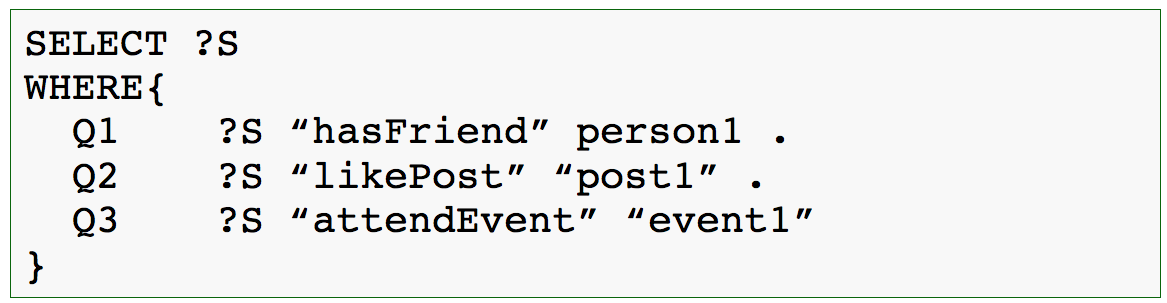
\includegraphics[width=0.5\textwidth]{figs/examplequery.png}
\end{center}
\vspace{-0.2in}
    \begin{center}
    	\includegraphics<1>[width=0.8\textwidth]{figs/implementation1.png}
    	\includegraphics<2>[width=0.8\textwidth]{figs/implementation2.png}
    \end{center}
\end{frame}


\begin{frame}
\frametitle{Outline}
	\begin{itemize}
		\item Introduction
		\item Query Decomposition and Data Partition
		\item Parallel and Distributed Query Planner
		\item Continuous Join
		\item Implementation
		\item Experiment Result
		\item \textcolor{blue!20}{Conclusion}
	\end{itemize}
\end{frame}

\begin{frame}
\frametitle{Experiment Setting}
\begin{itemize}
\item We evaluate the system on Grid 5000, with 11 nodes. 1 Master (Nimbus), 10 Slaves (Supervisor). 

\item The Storm version is 1.0, and we only use one slot on each machine.

\item Apache Jena API is used for reading triples.
\end{itemize}

\end{frame}

\begin{frame}
\frametitle{Data sets}
\begin{itemize}
\item Synthetic data
\begin{itemize}
\item The RDF triples generated in Spouts are distributed to the nodes according to their predicate. 
\item Two sub-sets of data are generated. The  first sub-set contains only the results of the join, and the second one contains only the non-results of the join.
\end{itemize}
\item LUBM Data 
\begin{itemize}
\item LUBM has 14 queries, and we have tested query No.1, query No.3, and query No.4
\item It consists of a university domain. 
\item It is customizable and repeatable.
\end{itemize}
\end{itemize}
\end{frame}

\begin{frame}
\frametitle{Evaluations}
\textbf{Impacts: (x axis)}
\begin{itemize}
\item Sliding Window Size
\item Number of Generations
\end{itemize}
\textbf{Metrics: (y axis)}
\begin{itemize}
\item Execution Latency --- The difference between the time an element is generated and the time it is emitted as a result
\item Process Latency --- The difference between the time an element is generated and the time it begins to be processed
\item Data Transmitted
\item Accuracy
\end{itemize}
\end{frame}

\begin{frame}
\frametitle{Execution Lateny}
\vspace{-0.1in}
Sliding Window Size = 800 (1V)
\vspace{-0.2in}
    \begin{center}
    	\includegraphics<1>[width=0.7\textwidth]{figs/II_1V_EL.png}
    \end{center}
\end{frame}

\begin{frame}
\frametitle{Execution Latency}
\vspace{-0.1in}
Number of Generation = 6 (1V)
\vspace{-0.2in}
\begin{center}
    	\includegraphics<1>[width=0.7\textwidth]{figs/III_1V_EL.png}
\end{center}
\end{frame}

\begin{comment}
\begin{frame}
\frametitle{Processing Lateny}
\vspace{-0.1in}
Sliding Window Size = 800 (1V)
\vspace{-0.2in}
    \begin{center}
    	\includegraphics<1>[width=0.7\textwidth]{figs/II_1V_PL.png}
    \end{center}
\end{frame}


\begin{frame}
\frametitle{Processing Latency}
\vspace{-0.1in}
Number of Generation = 6 (1V)
\vspace{-0.2in}
\begin{center}
    	\includegraphics<1>[width=0.7\textwidth]{figs/III_1V_PL.png}
\end{center}
\end{frame}
\end{comment}

\begin{frame}
\frametitle{Data Transmitted -- Sliding Window Size = 800}
\begin{columns}
\begin{column}{0.5\textwidth}
1V
 	\includegraphics<1>[width=1\textwidth]{figs/II_1V_DT.png}
\end{column}
\begin{column}{0.5\textwidth}
MV
 	\includegraphics<1>[width=1\textwidth]{figs/II_MV_DT.png}
\end{column}
\end{columns}
400 more data transmission without Bloom Filters.
\end{frame}

\begin{frame}
\frametitle{Accuracy}
\textbf{We got 100\% correct results --- Surprise!}

\begin{itemize}
\item use p (false positive rate) and n (number of element to be inserted) to decide m (number of bits in the Bloom Filter)

\item n is set to the number of elements received by the triple pattern

\item the real number of elements inserted into the Bloom Filter should be the number of results which match the triple pattern (far less than n)
\end{itemize}

%Because we use p and n to decide m. Each time n is set to the number of elements contained by each generation, but actually, the real number of elements inserted into the Bloom Filter should be the number of results which match the triple pattern, which is much less then what we set. Since each time we set p to 0.05\%, which is rather small, we didn't get any false positive results in our experiments.
\end{frame}

\begin{frame}
\frametitle{Outline}
	\begin{itemize}
		\item Introduction
		\item Query Decomposition and Data Partition
		\item Parallel and Distributed Query Planner
		\item Continuous Join
		\item Implementation
		\item Experiment Result
		\item Conclusion
	\end{itemize}
\end{frame}

\begin{frame}
\frametitle{Conclusion}
\begin{itemize}
\item Parallel and distributed join processing on RDF streams
\item Distribute both data and queries
\item Efficient
\begin{itemize}
\item Time 
\begin{itemize}
\item Execution Latency less than 600 ms
\item Process Latency less than 1 ms
\end{itemize}
\item Space --- 400 times more efficient than without using Bloom FIlters
\end{itemize}
\end{itemize}
\end{frame}

\begin{comment}
\begin{frame}
\frametitle{Conclusion}
\vspace{-0.1in}
	\begin{itemize}
		\item Query Decomposition and Data Partition
		\begin{itemize}
		\item[-] According to predicate
		\end{itemize}
		\item Parallel and Distributed Query Planner
		\begin{itemize}
		\item[-] use Bloom Filter to communicate among sub-queries
		\item[-] 3 types of different kinds of joins according to the structure
		\item[-] one rule for communication order
		\end{itemize}
		\item Continuous Join
		\begin{itemize}
		\item[-] Sliding Window + Sliding Bloom Filter
		\end{itemize}
		\item Analysis
		\begin{itemize}
		\item[-] Bloom Filters
		\item[-] Dominating Parameters for the System
		\end{itemize}
		\item Implementation
		\begin{itemize}
		\item[-] Spout + BuilderBolt + ProberBolt
		\end{itemize}
		\item Experiment Result
		\begin{itemize}
		\item[-] Processing Latency + Execution Latency + Data Transmission
		\end{itemize}
	\end{itemize}
\end{frame}
\end{comment}
%!TEX root = presentazionelancia.tex
\section{Conclusion and Future Work}
\begin{frame}
\frametitle{Implementation}
To achieve performance and storage efficiency Fb have implemented some optimizations to servers.  
\end{frame}

\begin{frame}[c]\frametitle{Caching Servers}
\begin{itemize}
	\item Memory is partitioned into arenas by association type
	\begin{itemize}
		\item This mitigates the issues of poorly behaved association types
		\item They can also change the lifetime for important associations
	\end{itemize}
	\item Small items with fixed size have a lot of pointer overhead
	\begin{itemize}
		\item stored separately
		\item Used for association counts
	\end{itemize}
\end{itemize}    
\end{frame}

\begin{frame}[fragile]\frametitle{MySql Mapping}
    We divided the space of objects and associations into \emph{shards}. Each \emph{shard}:
    \begin{itemize}
    	\item is assigned to a logical DB
    	\item there is a table for objects and a table for associations
    	\item all field of object are serialized in a single \verb!data! column
    	\item object of different size can be stored in the same column
    \end{itemize}
Exceptions:
\begin{itemize}
	\item Some object can benefit from being stored in a different table
	\item Associations counts are stored in a separate table
\end{itemize}
\end{frame}

\begin{frame}[c]\frametitle{Cache Sharding}
    Shards are mapped to chache server using consistent hashing (like dynamo)

    This can lead to \emph{imbalances}, so TAO use shard cloning to rebalance the load

    There are also \emph{popular object} that can be queried a lot more often than others.

    TAO says to the clients to cache them these objects
\end{frame}

\begin{frame}[fragile]\frametitle{High-Degree Objects}
    Some object have a lot of associations (remember there were a limit of 6000?)
    \begin{itemize}
    	\item TAO can't cache all associations list
    	\item Requests will always end to Db
    \end{itemize}
    so
    \begin{itemize}
    	\item For \verb!assoc_count!, the edge direction is chosen using the lower degree between source and destination object
    	\item For \verb!assoc_get! query, only associations whose time~ >~ object's ~creation~ time
    \end{itemize}




\end{frame}
%%!TEX root = presentazionelancia.tex
\section{Consistency \& Failures}
\begin{frame}[t]\frametitle{Consistency}
	Under normal operation, TAO is \emph{eventually consistent}

	Replication lag usually < 1"

	Race conditions are resolved by using version numbers

	In special ``\emph{critical}" situation a read can be forwarded to database to ensure to read from a consistent source of truth. (Useful for auth procedures)

\end{frame}

\begin{frame}[t]\frametitle{Detecting Failures}
    Each TAO server stores per-destination time-outs
    \begin{itemize}
    	\item if several time-outs occur, hosts are marked as down
    	\item subsequent requests are aborted
    	\item Tao reacts trying to route around failures (favouring availability over consistency)
    	\item Down hosts are actively probed to check if recover
    \end{itemize}
\end{frame}

\begin{frame}[c]\frametitle{Handling Failures}
    \begin{description}
    	\item[Database Fail] Db can crash or be off-line for maintenance. 
    	\begin{itemize}
    		\item If master db is down, a slave is promoted to new master
    		\item If a slave db is down, cache miss are redirected to TAO leaders in master region
    	\end{itemize}
    	\item[Leader Fail] Followers re-route requests around it
    	\begin{itemize}
    		\item Read miss goes directly to db
    		\item Write are routed to a random member of the leader tier
    	\end{itemize}
    \end{description}
\end{frame}

\begin{frame}[c]\frametitle{Handling Failures (2)}
    \begin{description}
    	\item[Invalidation Fail] Leader can't contact a follower during a cache invalidation message
    	\begin{itemize}
    		\item Leader queues message 
    		\item If Leader also crash message are lost so new leader send bulk invalidation
    	\end{itemize}
    	\item[Follower Fail] Followers in others tiers share the responsibility of it's shard
    	\begin{itemize}
    		\item Tao client have a primary tier and a backup tier
    	\end{itemize}
    \end{description}


\end{frame}

%input{workload}

\setbeamercolor{background canvas}{bg=matblue}
\setbeamercolor{normal text}{fg=white}
\begin{frame}[plain, b]
\centering
\huge \textcolor{white}{Thank You!}
\normalsize

\vspace*{\fill}

 \begin{beamercolorbox}[wd=\paperwidth]{section in head/foot}
 \centering
Parallel and Continuous Join Processing for Data Stream
\vskip10pt
\end{beamercolorbox}
 \end{frame}

\end{document}
